\documentclass[11pt,letterpaper]{article}
\usepackage{graphics}
\usepackage{fullpage}
\addtolength{\voffset}{0.5in}

%
%  Cool LaTeX resource:
%   http://en.wikibooks.org/wiki/LaTeX

\begin{document}
\title{Self-improving tutor system}
\author{Brett van de Sande}

% Assignment of blame paper: 
% http://www.public.asu.edu/~kvanlehn/Stringent/PDF/07UM_KVL_KK_etal.pdf
%   my ``opportunity'' equals their ``step''
%   my ``turn'' equals their ``transaction''
%
% Doing reinforcement learning by direct policy search.
% See discussion on p. 17 of:
% http://www.cs.brown.edu/research/pubs/theses/phd/2002/peshkin.pdf


\maketitle

\section{A model of learning}

For each student and KC, the student has attempted some number of 
{\em steps} that involve a given skill.   We will label
steps with $j$.  Usually a given step is associated
with a single user interface object (an equation, vector, etc.)  but
not always, since a student may attempt a particular problem solving
step, delete the object, and later attempt that solution step again.
Each step $j$ corresponds some some number of student {\em transactions}:
attempts at constructing the associated object, or associated
interactions with the Andes help system.  

Next, we need of student learning for a particular KC.
Since the policies chosen by the random-help version of Andes
are different for each student,
we need to determine the point of learning for each student.
For each KC and student, mark each step as ``correct'' if
the student completes the step correctly without any associated errors or 
requests for help; otherwise, the step is marked as ``incorrect.''


\section{Objective function}



The objective function is 
\begin{eqnarray}
  Z&=&\sum_{\mbox{student, KC, policy}} \sum{j}  \frac{P^*_j}{n_j}
  \sum_{k\in \sigma_j} \left(f(\mathbf{x}_k)-d_k\right))^2 \\
 &&+\frac{1-P*^*_j}{n_j}
  \sum_{k\in \sigma_j} \left(f(\mathbf{x}_k)-(1-d_k)\right)^2 + \\
\end{eqnarray}
where $P_j^*$, $n_j$, $\mathbf{x}_k$, and $d_k$ are understood to be
functions of student, KC, and tutor policy.  $d_k\in \{0,1\}$ is the
policy actually taken by the random-help version of Andes for transaction
$k$.  
$\sigma_j$ is the set of transactions associated with step $j$ 
and $n_j$ is the associated number of turns
taken.  Finally, $P^*_j$ is the probability that the student learned the
given skill, given that they haven't learned it already.


\section{Models of learning}

A number of authors have used a logistic funtion, 
${\mathrm logit}(x)=(1+\tanh(x/2))/2$, to 
model student learning.  In that case, we have a two-parameter
model for the probability that the student gets step $j$ correct:
%
\begin{equation}
               P_j^{\mathrm logit} = {\mathrm logit}\left(\beta (j-L)\right)
\end{equation}
%
where $\beta$ is the steepness of the function and $L$ is the moment
of learning.

Alternatively, we can use a function that retains the 
guess $P(G)$ and slip $P(S)$ probabilities of Corbett and Anderson~\cite{anderson}.
The simplest such model is a step:
\begin{equation}
               P_j^{\mathrm step} = \left\{\begin{array}{cc}
                                       P(G),& j<L\\
				       1-P(S),& j\ge L
                                    \end{array}\right. \label{step}
\end{equation}
%
\[
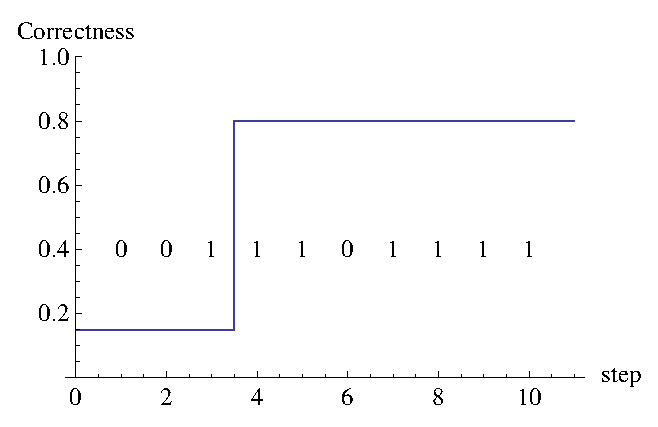
\includegraphics{step.eps}
\]
We can match $P_j^{\mathrm step} $ to the student data using the
Maximun Likelihood method.
Let $c_i$ \& $w_i$ be the number of correct \& incorrect steps observed
for $j<L$ and $c_f$ \& $w_f$ be the number of correct \& incorrect
steps for $j\ge L$.  The associated log likelihood for a given $L$ is
%
\begin{eqnarray}
  \mathcal{L}_L = &\sum_j & \log\left(P(G)^{c_i} \left(1-P(G)\right)^{w_i}\right) 
                      + \log\left(P(S)^{w_f} 
                     \left(1-P(S)\right)^{c_f} \right)  \nonumber \\
                   & &+(\mbox{normalization constant}) \, .
\end{eqnarray}
Note that the guess and slip rates follow the binomial distribution.
$\mathcal{L}_L$ is maximized when:
%
\begin{eqnarray}
  P(G) &=&  \frac{c_i}{c_i+w_i} \, ,\\
  P(S) &=&  \frac{w_f}{c_f+w_f} \,  .
\end{eqnarray}
%
Next, on can maximize $\mathcal{L}_L$ with respect to $L$ to find
the most likely value $L=L_\mathrm{max}$.  However, in practice, the 
uncertainty in $L$ can be significant and is often not normally
distributed.   Instead we will consider a set of models, each with a 
different value of $L$, and a relative probability given by AIC ~\cite{aic-book}.  That
is, the model for each value of $L$ has weight,
%
\begin{equation}
                   w_L = \frac{\mathrm{e}^{\mathcal{L}_L-2} }{W}\, ,
\end{equation}
with normalization $W$ such that $\sum_L w_L=1$.

Finally, we need to determine whether learning has occurred.  Thus,
we demand that the step in~(\ref{step}) is increasing: $P(S)+P(G) <1$.



\section{Baysian Knowledge tracing}

The Bayesian Knowledge tracing model~\cite{anderson} has four parameters:
%
\begin{itemize}
   \item $P_0$ is the initial probability of knowing a skill.
   \item $P(G)$ is probability of guessing correctly, if the student        
         doesn't know the skill.
   \item $P(S)$ is probability of slips, if student does know the skill.
   \item $P(L)$ is probability of learning the skill if the student 
         does not know the skill.  Note that this is assumed to 
         be constant over steps.
\end{itemize}
%
Let $P_j$ be the probability that the student knows the skill at 
step $j$. According to the model,  $P_j$ can
be determined in terms of the previous opportunity:
%
\begin{equation}
          P_j = P_{j-1} + P(L)\left(1-P_{j-1}\right)
\end{equation}
%
According to this model, the probability that the student actually gets
opportunity $n$ correct is:
%
\begin{equation}
         P_j(C) = P(G)\left(1-P_j\right) + \left(1-P(S)\right) P_j \label{pnc}
\end{equation}
%
(Unlike the four model parameters above, there isn't a consistent
notation for $P_j(C)$ in the literature.)
This model can be exactly solved with solution: 
%
\begin{equation}
            P_j = 1-\left(1-P(L)\right)^j\left(1-P_0\right)
	    \label{sol}
\end{equation}
%
%
Substituting (\ref{sol}) into (\ref{pnc}), we get:
%
\begin{equation}
         P_j(C) = 1-P(S) -\left(1-P(S)-P(G)\right) \left(1-P_0\right)
                   \left(1-P(L)\right)^j \label{pncsoln}
\end{equation}
%
Note that the functional form of $P_j(C)$ is a function of {\em three}
parameters:  $P(S)$, $P(L)$, and $\left(1-P(S)-P(G)\right) \left(1-P_0\right)$.
This degeneracy of the model was first noticed by Beck and 
Chang~\cite{beckchang}.  In their paper, they notice that multiple
combinations of $P(G)$ and $P_0$ give exactly the same $P_j(C)$, but
fail to explain why this is the case.

The functional form of (\ref{pncsoln}) is an exponential.
If we define 
$A=\left(1-P(S)-P(G)\right) \left(1-P_0\right)$ and
$\beta=-\log(1-P(L))$, then we can rewrite (\ref{pncsoln}) in 
a clearer form:
%
\begin{equation}
         P_j(C) = 1-P(S) -A e^{-\beta j}
\end{equation}
%
So the graph of  $P_j(C)$ looks like the following:
%
\[
\includegraphics{exponential.eps}
\]

There are several conclusions for our project:
\begin{enumerate}

  \item The functional form of $P_j(C)$ (and of $P_j$) means that
  the biggest change in learning always occurs in the first
  opportunity and decreases monotonically after that.  So, using
  this model to determine where the greatest learning
  occurred is pointless.

  \item Is $P_n(C)$ better than the step-function model that I
  introduced?  Both are three-parameter models that are 
  to be fitted to the log data.  The real question is which
  model better fits, on average, the log data?  That is something
  that can only be determined experimentally.

  \item Probably the most appropriate method of fitting
  $P_j(C)$ to the log data is by using Maximum Likelihood.
  I looked into finding a partial algebraic solution, but
  the equations are too complicated.  Thus, one would need
  to calculate the three model parameters numerically.

\end{enumerate}

\begin{thebibliography}{9}

\bibitem{anderson} 
  Corbett, A.\ T., Anderson, J.\ R. Knowledge Tracing:  Modeling 
the Acquisition of Procedural Knowledge.  \emph{User Modeling and
 User-Adapted Interaction}, 1995, 4, 253--278.

\bibitem{beckchang}
  Beck, J.\ E., Chang, K.-m.\ Identifiability: A Fundamental Problem of
  Student Modeling.
  \emph{Proceedings of the $11^{th}$ International Conference on User 
    Modeling}, 2007.

\bibitem{aic-book}Burnham, K.~P., and Anderson, D.~R. \emph{Model
  Selection and Multimodel Inference: A Practical
  Information-Theoretic Approach}, 2nd ed. Springer-Verlag. 2002.

\end{thebibliography}




\end{document}